\section{Hybrid Metaheuristc}


A large  number of researchers have recognized the advantages and huge potential Building
hybrid mathematical programming methods and metaheuristics.
The main motivation to create hybrid Metaheuristics is to exploit the complementary character of different optimization strategies. In fact, choosing an adequate combination of algorithmic can be the key for achieving top performance in solving many hard optimization problems \cite{Puchinger2005} \cite{Blum2012}.


There are two main categories of metaheuristc combinations: Collaborative Combinations and Integrative Combinations. The Fig. \ref{fig:metaheuristc} presents the two main categories of Hybrid MetaHeuristc \cite{Puchinger2005}.

\begin{figure}[h]
\caption{Categories of metaheuristc combinations \cite{Puchinger2005} }
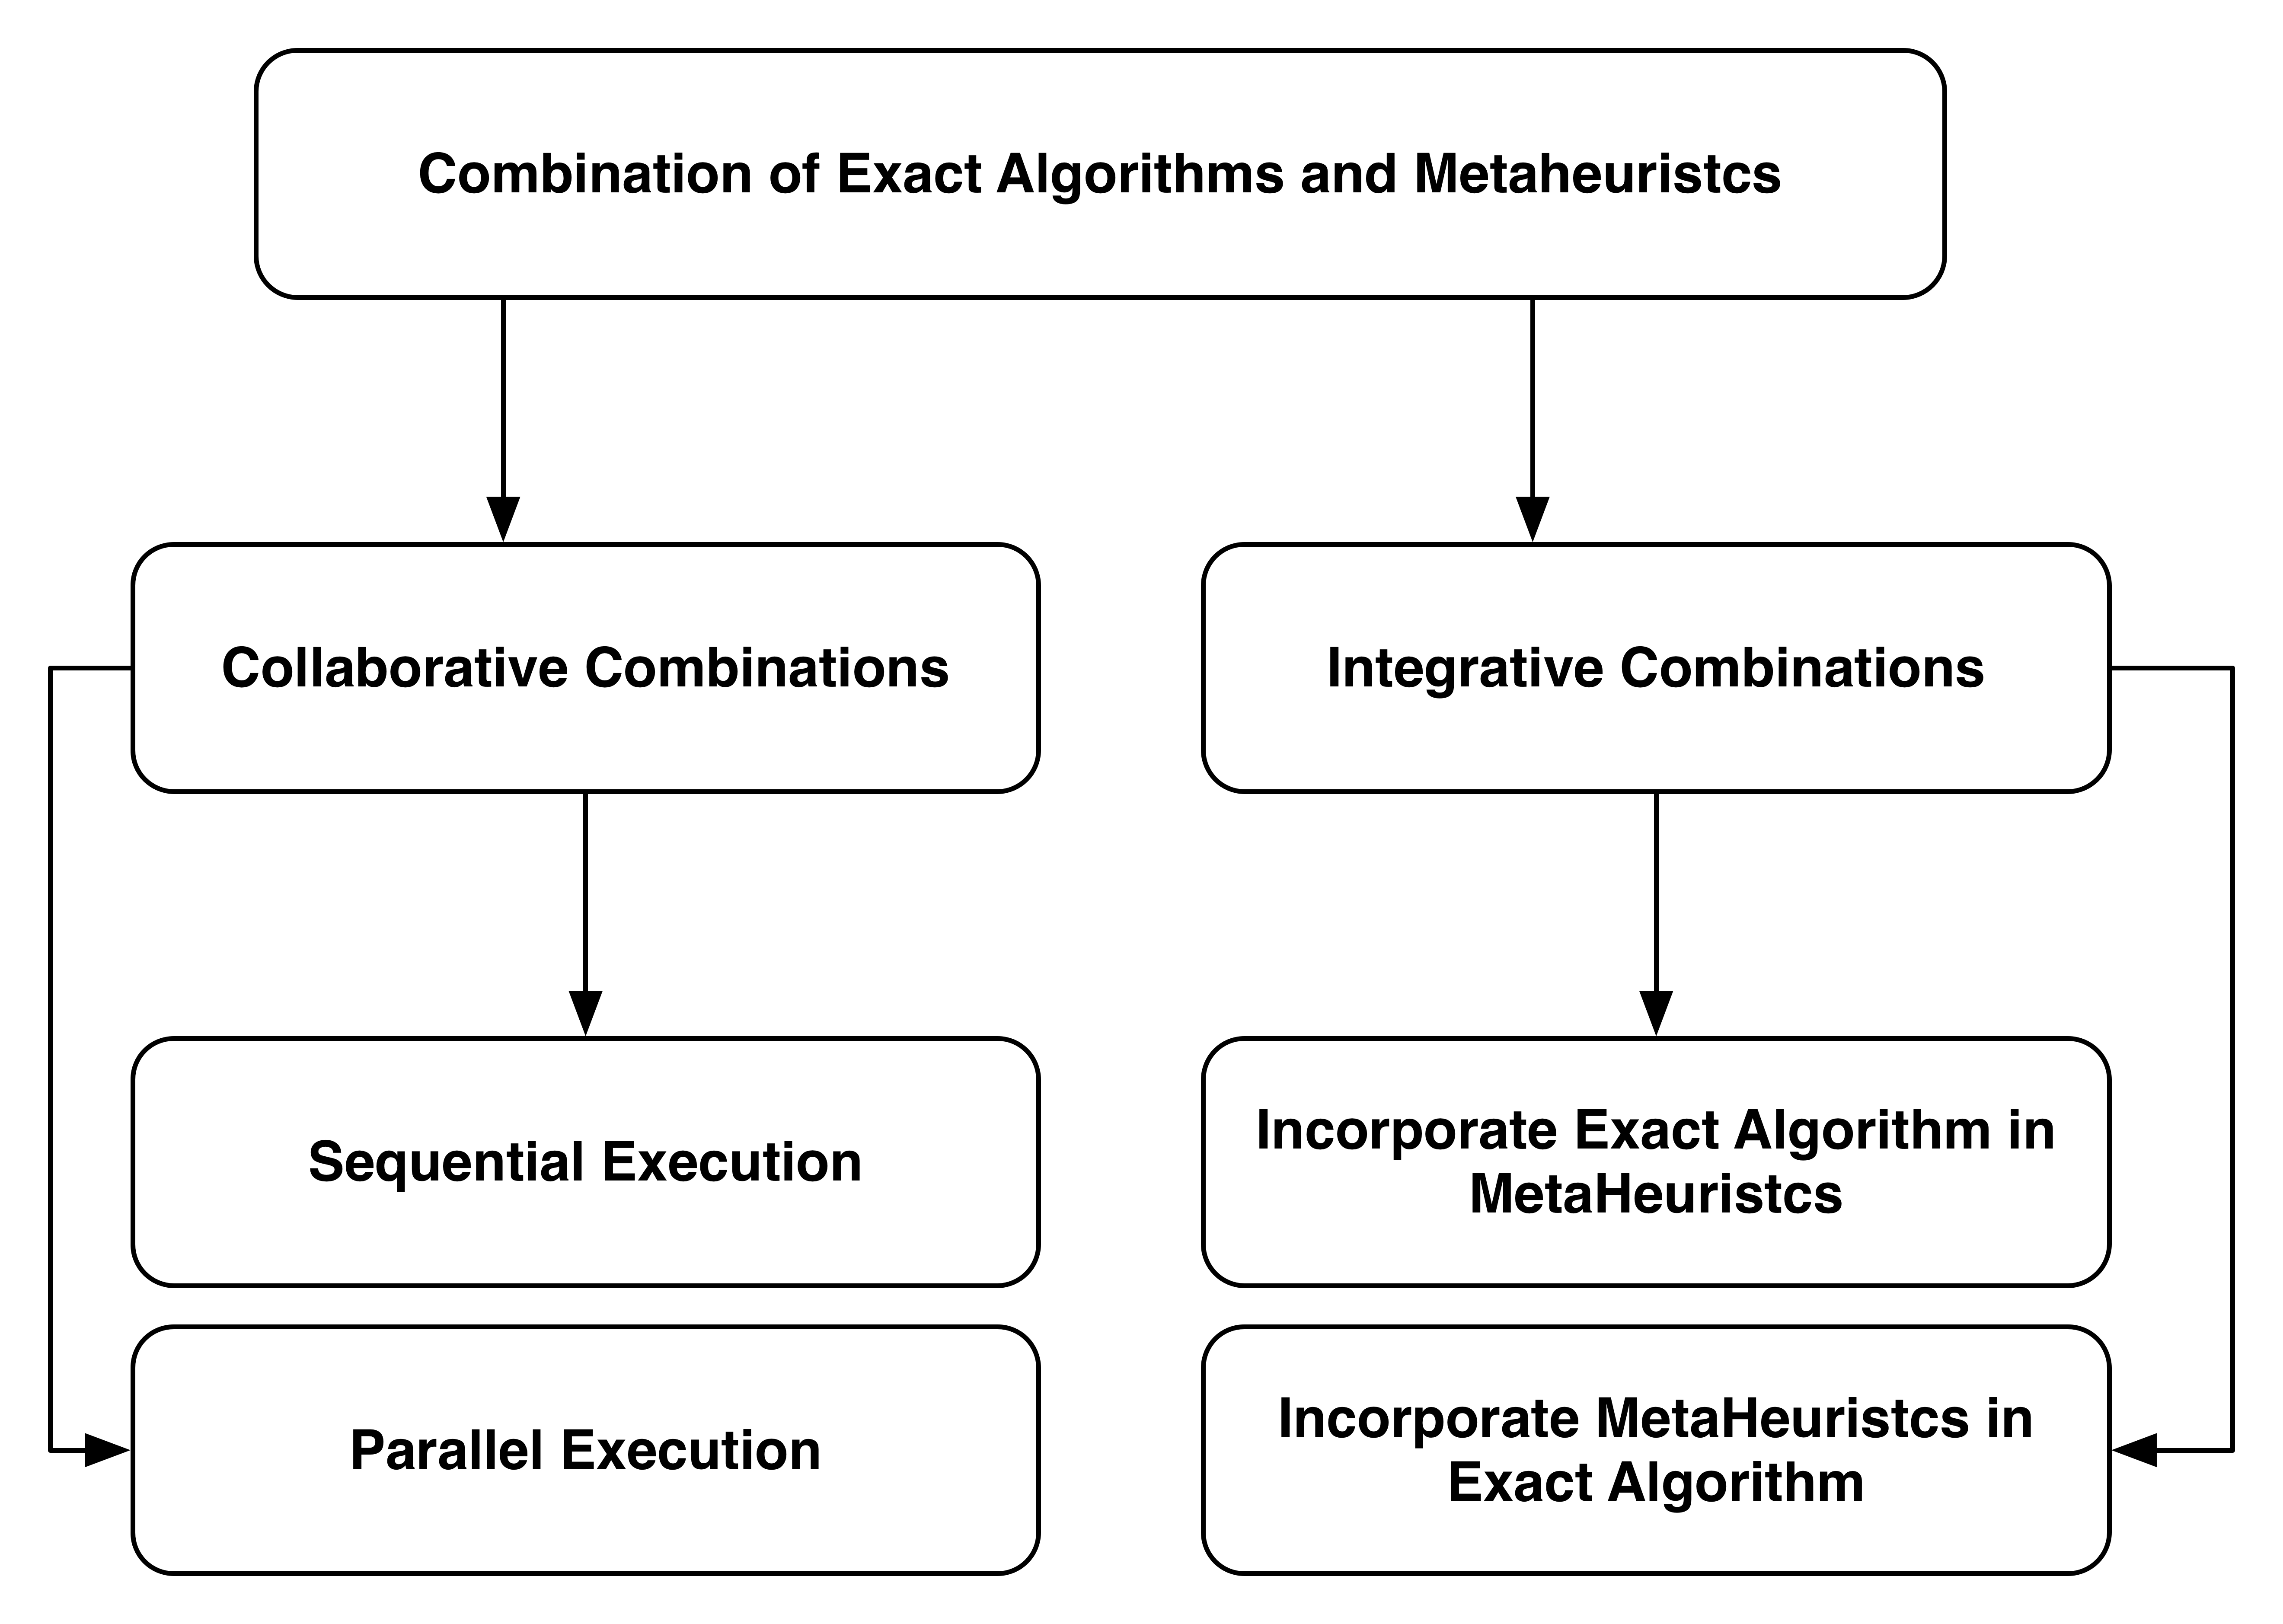
\includegraphics[width=0.5\textwidth]{./images/metaheuristcs.png}
\label{fig:metaheuristc}
\end{figure}

Collaborative Combinations uses a approach where the  algorithms exchange information, but are not part of each other. In this approach,  algorithms may be executed sequentially or in parallel.

A common Collaborative Combination approach used in Hybrid Metaheuristc is the Population-Based Iterated Local Search.
The Listing \ref{pbils} shows a example of algorithm that  uses  Population-Based Iterated Local Search.  The algorithm starts  creating a population of n individuals. A local search is applied to all individuals s $\in$ P. The algorithm performs a loop where a perturbation creates new individuals. These individuals are added to an auxiliary variable P'.  Finally , the algorithm selects the best n individuals of P'.

\lstdefinestyle{outline}{
		language=Java,
         basicstyle=\scriptsize\ttfamily,
         numberstyle=\tiny,
         numbersep=5pt,
         tabsize=2,
         extendedchars=true,
         breaklines=true,
         keywordstyle=\color{black}\bf,
         frame=b,  % <<<<<<<<<<<<<<<<<<<<<<<<<<
         stringstyle=\color{green!40!black}\ttfamily,
         showspaces=false,
         showtabs=false,
         literate=
               {=}{$\leftarrow{}$}{1}
               {==}{$={}$}{1}
               {ee}{$\in{}$}{1}
               {union}{$\cup$}{1},
         numbers=left,
         xleftmargin=17pt,
         framexleftmargin=17pt,
         framextopmargin=1pt, % <<<<<<<<<<<<<<<<<<<<<<
         showstringspaces=false,
         %backgroundcolor=\color[RGB]{200,200,200},
         belowcaptionskip=0pt,
         mathescape=true
}


\begin{lstlisting}[style=outline,caption={Population-Based Iterated Local Search},float,label=pbils]
P=GenerateInitialPopulation(n) 
Apply LocalSearch() to all s ee P
while termination conditions not met do 
	P'=P
    for all s ee P do
	    s'=Perturbation(s,history) 
    	s''= LocalSearch(s') 
        P' ←P' union {s''}
    end for
    P= Best n solutions from P
end while    
\end{lstlisting}

% * <naubergois@gmail.com> 2015-09-17T00:47:43.344Z:
%
%  Rever explicacacao do algoritmo
%


